\section{第九周数值分析实验}
\subsection{正交函数族最佳平方逼近}
\begin{ex}
	设 $f(x)=\frac{1}{1+25 x^2}, x \in[-1,1]$, 利用勒让德正交多项式族, 分别构造 $3$ 次, $6$ 次, $10$ 次最佳平方逼近多项式, 并绘图与 $f(x)$ 比较.
\end{ex}
\lstinputlisting[language=matlab]{w9/legendremap.m}
\lstinputlisting[language=matlab]{w9/work9q1.m}
\qa 
\begin{flalign*}
	\begin{split}
		S_3(x)=\left(\frac{9}{20}-\frac{21\,\mathrm{atan}\left(5\right)}{25}\right)\,x^2+\frac{12\,\mathrm{atan}\left(5\right)}{25}-\frac{3}{20}.
	\end{split}&
\end{flalign*}
\begin{flalign*}
	\begin{split}
		S_6(x)=&\left(\frac{6579573}{250000}-\frac{28501473\,\mathrm{atan}\left(5\right)}{1250000}\right)\,x^6+\left(\frac{1102563\,\mathrm{atan}\left(5\right)}{31250}-\frac{1988679}{50000}\right)\,x^4\\&+\left(\frac{787143}{50000}-\frac{3698793\,\mathrm{atan}\left(5\right)}{250000}\right)\,x^2+\frac{166579\,\mathrm{atan}\left(5\right)}{125000}-\frac{52633}{50000}.
	\end{split}&
\end{flalign*}
\begin{flalign*}
	\begin{split}
		S_{10}(x)=&\left(\frac{15053862021341}{15000000000}-\frac{37844796458469\,\mathrm{atan}\left(5\right)}{50000000000}\right)\,x^{10}+\left(\frac{4806364476771\,\mathrm{atan}\left(5\right)}{2500000000}-\right.\\&\left.\frac{4448386331961}{1750000000}\right)\,x^8+\left(\frac{1145902042857}{500000000}-\frac{8707875715539\,\mathrm{atan}\left(5\right)}{5000000000}\right)\,x^6\\&+\left(\frac{1668177980469\,\mathrm{atan}\left(5\right)}{2500000000}-\frac{217491363947}{250000000}\right)\,x^4+\left(\frac{123339641139}{1000000000}-\right.\\&\left.\frac{970103687553\,\mathrm{atan}\left(5\right)}{10000000000}\right)\,x^2+\frac{19197012681\,\mathrm{atan}\left(5\right)}{6250000000}-\frac{1037189439}{312500000}.
	\end{split}&
\end{flalign*}
\begin{figure}[H]
	\centering
	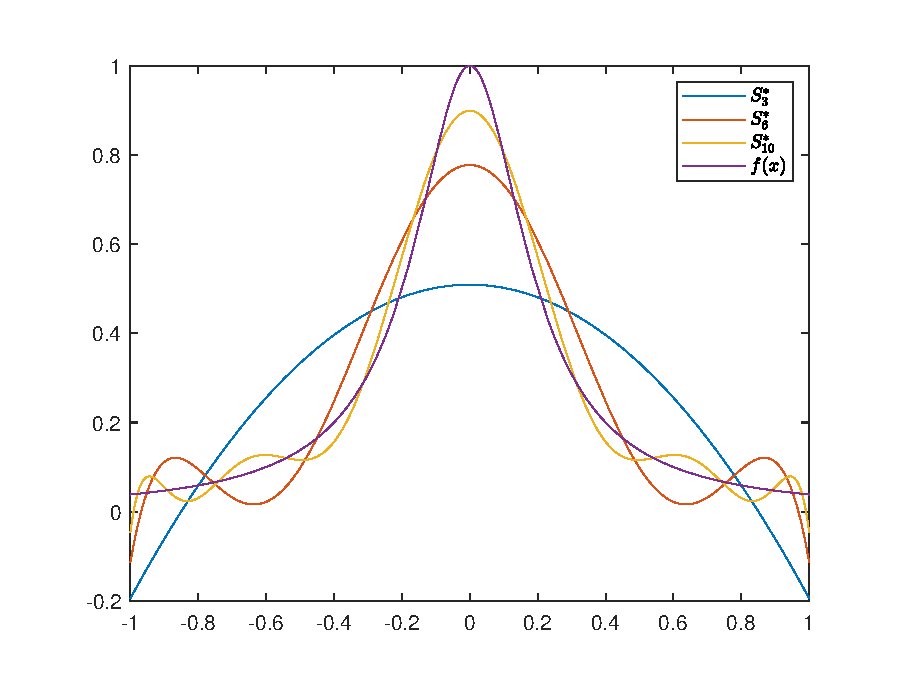
\includegraphics[width = 0.61\linewidth]{w9/figq1.eps}
	\caption{最佳平方逼近}
\end{figure}
\subsection{最小二乘拟合}
\begin{ex}
	实验数据如下
	
	\begin{tabular}{|c|c|c|c|c|c|c|c|c|c|c|c|c|}
		\hline$x_i$ & -1 & -0.8 & -0.6 & -0.4 & -0.3 & -0.1 & 0 & 0.2 & 0.4 & 0.6 & 0.8 & 1 \\
		\hline $y_i$ & 0 & 1.27 & 2.16 & 2.86 & 3.44 & 3.87 & 4.15 & 4.37 & 4.51 & 4.58 & 4.62 & 4.64 \\
		\hline
	\end{tabular}
	
	(1) 确定法方程组, 并求$ 2 $次及$ 3 $次拟合多项式函数 $s=s(x)$;
	
	(2) 与MATLAB拟合工具箱cftool对比.
\end{ex}
\lstinputlisting[language=matlab]{w9/work9q2.m}
\qa 
\begin{flalign*}
	\begin{split}
		y=-\frac{3982742614460357\,x^2}{2251799813685248}+\frac{2439825684435733\,x}{1125899906842624}+\frac{2288943766543947}{562949953421312}.
	\end{split}&
\end{flalign*}
\begin{flalign*}
	\begin{split}
		y=\frac{8521429937993895\,x^3}{18014398509481984}-\frac{7918081977677879\,x^2}{4503599627370496}+\frac{4129100537421519\,x}{2251799813685248}+\frac{4568116039683039}{1125899906842624}.
	\end{split}&
\end{flalign*}
\begin{figure}[H]
	\centering
	\subfloat[二次拟合多项式]{\includegraphics[width = 0.5\linewidth]{w9/figq21.eps}}
	\hfill
	\subfloat[三次拟合多项式]{\includegraphics[width = 0.5\linewidth]{w9/figq22.eps}}
	\hfill
	\subfloat[二次拟合多项式]{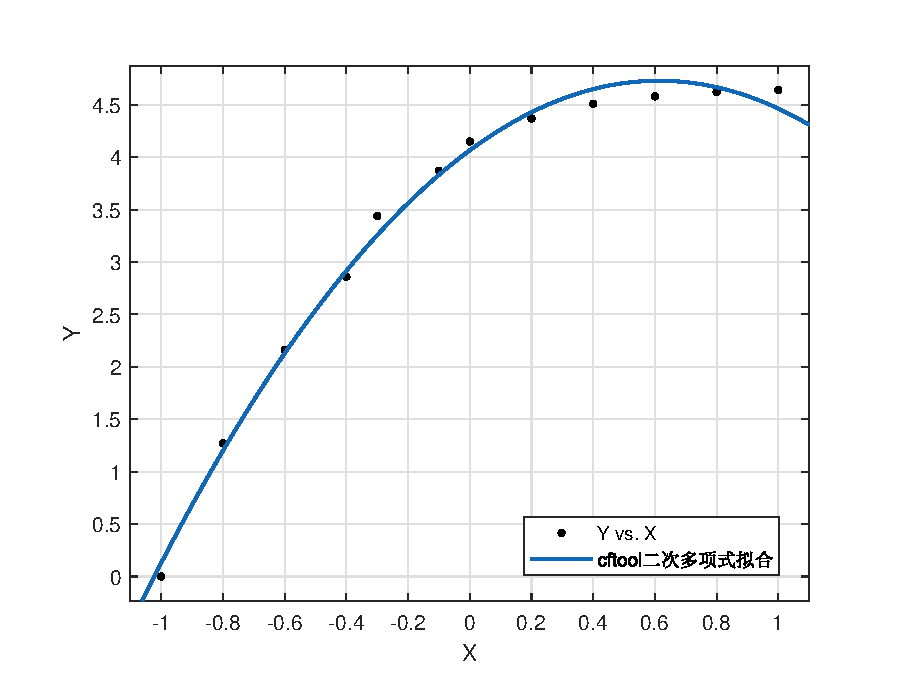
\includegraphics[width = 0.5\linewidth]{w9/figq2c1.eps}}
	\hfill
	\subfloat[三次拟合多项式]{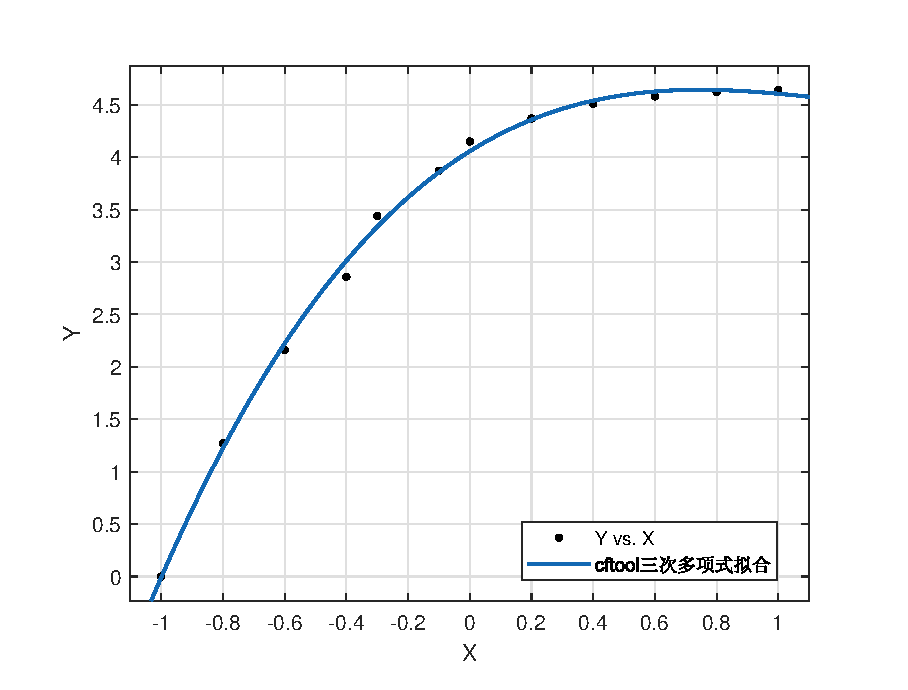
\includegraphics[width = 0.5\linewidth]{w9/figq2c2.eps}}
	\caption{最小二乘拟合}
\end{figure}
